% =============================================================================
% Chapter 5: Multi-Modal Sensor Fusion Framework
% =============================================================================
\selectlanguage{hebrew}

\section{מסגרת מיזוג חיישנים רב-מודאלית}
\label{sec:ch05_fusion}

\subsection{מבוא למיזוג חיישנים תרמי-חזותי}
\label{sec:ch05_intro}

מיזוג מידע מחיישנים מרובים הוא אבן יסוד במערכות ניווט אוטונומיות עמידות. בעוד שכל חיישן בודד מציג מגבלות ייחודיות, השילוב הנכון של חיישנים משלימים יכול לספק מודעות מצבית חזקה משמעותית מזו שמספק כל חיישן בנפרד. במקרה של ניווט רחפנים לילי, השילוב בין מצלמה חזותית (\en{RGB}) למצלמה תרמית (\en{IR}) הוא טבעי במיוחד: המצלמה החזותית מספקת רזולוציה מרחבית גבוהה ומידע מרקם עשיר בתנאי תאורה טובים, בעוד שהמצלמה התרמית מספקת מידע שימושי גם בחושך מוחלט, אם כי ברזולוציה נמוכה יותר ורעש גבוה יותר.

בפרק זה אנו מציגים מסגרת מיזוג רב-שכבתית (\en{multi-level fusion framework}) הפועלת בשלוש רמות שונות: רמת פיקסלים (\en{pixel-level fusion}), רמת תכונות (\en{feature-level fusion}), ורמת החלטה (\en{decision-level fusion}). המסגרת כוללת מנגנון קשב צולב (\en{cross-attention mechanism}) חדשני המאפשר לרשת המיזוג להתמקד באופן דינמי במידע הרלוונטי מכל מודאליות. בנוסף, אנו מציגים מנגנון מיזוג אדפטיבי מבוסס תנאי תאורה, המתאים את משקל התרומה של כל חיישן בהתאם לתנאי הסביבה.

\subsection{מיזוג ברמת פיקסלים}
\label{sec:ch05_pixel_fusion}

מיזוג ברמת פיקסלים הוא הרמה הבסיסית ביותר של מיזוג חיישנים, הפועלת ישירות על ערכי הפיקסלים בתמונה. שיטה זו דורשת רישום מרחבי מדויק בין התמונות משתי המודאליות, כפי שתואר בפרק הקודם. לאחר הרישום, כל פיקסל בתמונה הממוזגת הוא פונקציה של הפיקסלים המקבילים בתמונה החזותית והתרמית.

השיטה הפשוטה ביותר היא מיזוג ממוצע משוקלל:

\begin{equation}
I_{\text{fused}}(\mathbf{p}) = \alpha \cdot I_{\text{vis}}(\mathbf{p}) + (1 - \alpha) \cdot I_{\text{ir}}(\mathbf{p})
\label{eq:ch05_weighted_average}
\end{equation}

כאשר $\alpha \in [0,1]$ הוא משקל המיזוג. שיטה פשוטה זו אינה מנצלת את מלוא הפוטנציאל של מיזוג חיישנים, שכן היא מתייחסת לכל הפיקסלים באותו אופן ואינה מתחשבת בתכונות המקומיות של התמונה.

שיטה מתקדמת יותר היא מיזוג מבוסס פירמידת לפלסיאן (\en{Laplacian pyramid fusion}), המפרקת כל תמונה למספר רמות תדר וממזגת כל רמה בנפרד. הפירוק לפירמידה מאפשר לשמר פרטים בתדר גבוה מהתמונה החזותית תוך שילוב מידע בתדר נמוך מהתמונה התרמית:

\begin{equation}
L_{\text{fused}}^{(k)} = G_{\alpha}^{(k)} \cdot L_{\text{vis}}^{(k)} + (1 - G_{\alpha}^{(k)}) \cdot L_{\text{ir}}^{(k)}
\label{eq:ch05_laplacian_pyramid}
\end{equation}

כאשר $L^{(k)}$ היא רמת הפירמידה ה-$k$, ו-$G_{\alpha}^{(k)}$ היא מפת משקלים מבוססת פעילות מקומית (\en{local activity map}) ברמה $k$.

\subsection{מיזוג ברמת תכונות עם מנגנון קשב צולב}
\label{sec:ch05_feature_fusion}

מיזוג ברמת תכונות פועל על ייצוגים מופשטים של התמונות, המופקים באמצעות רשת נוירונים עמוקה. גישה זו גמישה יותר ממיזוג ברמת פיקסלים, שכן היא מאפשרת לרשת ללמוד אילו תכונות חשובות מכל מודאליות עבור המשימה הספציפית.

הארכיטקטורה המוצעת מבוססת על מנגנון קשב צולב (\en{cross-attention}) בהשראת מודל ה-\en{Transformer}. הרשת מורכבת משני מקודדים (\en{encoders}) נפרדים, האחד לתמונות חזותיות והשני לתמונות תרמיות, המייצרים מפות תכונות $\mathbf{F}_{\text{vis}} \in \mathbb{R}^{H \times W \times D}$ ו-$\mathbf{F}_{\text{ir}} \in \mathbb{R}^{H \times W \times D}$ בהתאמה.

מנגנון הקשב הצולב מאפשר לכל מיקום מרחבי במודאליות אחת "לשאול" מידע מהמודאליות האחרת. עבור כל פיקסל $\mathbf{p}$, מנגנון הקשב מחושב כ:

\begin{equation}
\mathbf{F}_{\text{fused}}(\mathbf{p}) = \text{Softmax}\l$e$f$t( \frac{\mathbf{Q}_{\text{vis}}(\mathbf{p})$$$ \mathbf{K}_{\text{ir}}^T(\mathbf{p})}{\sqrt{d_k}} \right) \mathbf{V}_{\text{ir}}(\mathbf{p}) + \text{Softmax}\l$e$f$t( \frac{\mathbf{Q}_{\text{ir}}(\mathbf{p})$$$ \mathbf{K}_{\text{vis}}^T(\mathbf{p})}{\sqrt{d_k}} \right) \mathbf{V}_{\text{vis}}(\mathbf{p})
\label{eq:ch05_cross_attention}
\end{equation}

כאשר $\mathbf{Q}_{\text{vis}} = \mathbf{W}_Q \mathbf{F}_{\text{vis}}$, $\mathbf{K}_{\text{ir}} = \mathbf{W}_K \mathbf{F}_{\text{ir}}$, $\mathbf{V}_{\text{ir}} = \mathbf{W}_V \mathbf{F}_{\text{ir}}$ הן הטלות לינאריות של מפות התכונות למרחב השאילתה (\en{query}), המפתח (\en{key}), והערך (\en{value}) בהתאמה. $d_k$ הוא ממד הייצוג.

הרשת המלאה כוללת מספר בלוקי קשב צולב המופעלים ברזולוציות שונות, ומאפשרת לכידת קורלציות מודאליות-חוצות בקני מידה מרחביים שונים. לאחר בלוקי הקשב, מפות התכונות הממוזגות מוזנות למפענח (\en{decoder}) המייצר את התמונה הממוזגת הסופית.

\subsection{מיזוג ברמת החלטה}
\label{sec:ch05_decision_fusion}

מיזוג ברמת החלטה פועל על הפלטים של מערכות קבלת החלטות עצמאיות הפועלות על כל מודאליות בנפרד. במקרה שלנו, כל מודאליות מפעילה מודל זיהוי מכשולים עצמאי, וההחלטות ממוזגות באמצעות כללי הצבעה או שיטות הסתברותיות.

שיטת המיזוג ברמת ההחלטה מבוססת על חוק בייס, המשלב את ההסתברויות המותנות מכל מודאליות:

\begin{equation}
$P(\text{מכשול} \mid I_{\text{vis}}, I_{\text{ir}})$ = \frac{$P(I_{\text{vis}} \mid \text{מכשול})$ $P(I_{\text{ir}} \mid \text{מכשול})$ P(\text{מכשול})}{$P(I_{\text{vis}}, I_{\text{ir}})$}
\label{eq:ch05_bayesian_fusion}
\end{equation}

בהנחת אי-תלות בין המודאליות בהינתן המטרה (\en{conditional independence}), הניחוח המקובל בספרות \cite{Julier1997CovarianceIntersection}, ניתן לפשט את הביטוי ל:

\begin{equation}
$P(\text{מכשול} \mid I_{\text{vis}}, I_{\text{ir}})$ \propto P(\text{מכשול}) \cdot P_{\text{vis}}(\text{מכשול} \mid I_{\text{vis}}) \cdot P_{\text{ir}}(\text{מכשול} \mid I_{\text{ir}})
\label{eq:ch05_bayesian_simplified}
\end{equation}

כאשר $P_{\text{vis}}$ ו-$P_{\text{ir}}$ הן ההסתברויות המותנות המוערכות על ידי מודלי הזיהוי העצמאיים.

\subsection{מסגרת מיזוג אדפטיבית מבוססת תנאי תאורה}
\label{sec:ch05_adaptive_fusion}

אחד החידושים המרכזיים של עבודה זו הוא מנגנון המיזוג האדפטיבי, המתאים באופן דינמי את משקל התרומה של כל מודאליות בהתאם לתנאי התאורה הסביבתיים. המנגנון מבוסס על רשת משקלים קטנה (\en{weighting network}) המקבלת כקלט מדדי איכות מכל מודאליות ומפיקה את משקלי המיזוג האופטימליים.

מדדי האיכות כוללים:
\begin{enumerate}
  \item עוצמת תאורה ממוצעת: $L_{\text{amb}} = \frac{1}{N} \sum_{\mathbf{p}} I_{\text{vis}}(\mathbf{p})$
  \item ניגודיות מקומית ממוצעת: $\sigma_{\text{vis}} = \frac{1}{N} \sum_{\mathbf{p}} \| \nabla I_{\text{vis}}(\mathbf{p}) \|$
  \item רמת רעש תרמי: $\sigma_{\text{ir}} = \text{std}(I_{\text{ir}})$ באזור אחיד
  \item מספר נקודות עניין שזוהו בכל מודאליות
\end{enumerate}

משקל המיזוג האדפטיבי מחושב כ:

\begin{equation}
\alpha(t) = \sigma\l$e$f$t( \mathbf{w}_\alpha^T \cdot [L_{\text{amb}}(t)$$$, \sigma_{\text{vis}}(t), \sigma_{\text{ir}}(t), N_{\text{feat}}^{\text{vis}}(t), N_{\text{feat}}^{\text{ir}}(t)] + b_\alpha \right)
\label{eq:ch05_adaptive_weight}
\end{equation}

כאשר $\sigma(\cdot)$ היא פונקציית הסיגמואיד, $\mathbf{w}_\alpha$ ו-$b_\alpha$ הם פרמטרים נלמדים של רשת המשקלים. המשקל $\alpha$ נמצא בתחום $[0,1]$, כאשר $\alpha \to 1$ בתנאי תאורה טובים (משקל גבוה למצלמה חזותית) ו-$\alpha \to 0$ בתנאי חושך (משקל גבוה למצלמה תרמית).

התמונה הממוזגת הסופית מחושבת כ:

\begin{equation}
I_{\text{fused}}(\mathbf{p}, t) = \alpha(t) \cdot I_{\text{vis}}(\mathbf{p}, t) + (1 - \alpha(t)) \cdot I_{\text{ir}}(\mathbf{p}, t)
\label{eq:ch05_adaptive_fused}
\end{equation}

\subsection{מיזוג במרחב המצב: פילטר קלמן מורחב}
\label{sec:ch05_ekf_fusion}

מעבר למיזוג ברמת התמונה, אנו מבצעים מיזוג גם במרחב המצב (\en{state space fusion}) באמצעות פילטר קלמן מורחב (\en{Extended Kalman Filter, EKF}). פילטר זה ממזג את אומדני המצב מכל מודאליות תוך התחשבות באי-הוודאויות היחסיות שלהן.

מודל התצפית המאוחד מוגדר כ:

\begin{equation}
\mathbf{z}_k = \left[\mathbf{z}_k^{\text{vis}} \\ \mathbf{z}_k^{\text{ir}}\right] = \mathbf{h}(\mathbf{x}_k) + \mathbf{v}_k, \quad \mathbf{v}_k \sim \mathcal{N}(0, \mathbf{R}_k)
\label{eq:ch05_observation_model}
\end{equation}

כאשר $\mathbf{z}_k^{\text{vis}}$ ו-$\mathbf{z}_k^{\text{ir}}$ הם וקטורי התצפית מכל מודאליות, $\mathbf{h}$ הוא מודל התצפית הלא-לינארי, ו-$\mathbf{R}_k$ היא מטריצת שונות הרעש המשותפת.

שלב החיזוי של ה-\en{EKF}:

\begin{equation}
\hat{\mathbf{x}}_{k|k-1} = \mathbf{g}(\mathbf{u}_k, \hat{\mathbf{x}}_{k-1|k-1})
\label{eq:ch05_ekf_predict}
\end{equation}

\begin{equation}
\mathbf{P}_{k|k-1} = \mathbf{G}_k \mathbf{P}_{k-1|k-1} \mathbf{G}_k^T + \mathbf{Q}_k
\label{eq:ch05_ekf_cov_predict}
\end{equation}

כאשר $\mathbf{g}$ הוא מודל התנועה, $\mathbf{G}_k = \partial \mathbf{g}/\partial \mathbf{x}$ היא מטריצת היאקובי של מודל התנועה, ו-$\mathbf{Q}_k$ היא מטריצת שונות רעש התהליך.

שלב העדכון:

\begin{equation}
\mathbf{K}_k = \mathbf{P}_{k|k-1} \mathbf{H}_k^T (\mathbf{H}_k \mathbf{P}_{k|k-1} \mathbf{H}_k^T + \mathbf{R}_k)^{-1}
\label{eq:ch05_kalman_gain}
\end{equation}

\begin{equation}
\hat{\mathbf{x}}_{k|k} = \hat{\mathbf{x}}_{k|k-1} + \mathbf{K}_k (\mathbf{z}_k - \mathbf{h}(\hat{\mathbf{x}}_{k|k-1}))
\label{eq:ch05_state_update}
\end{equation}

\begin{equation}
\mathbf{P}_{k|k} = (\mathbf{I} - \mathbf{K}_k \mathbf{H}_k) \mathbf{P}_{k|k-1}
\label{eq:ch05_cov_update}
\end{equation}

כאשר $\mathbf{H}_k = \partial \mathbf{h}/\partial \mathbf{x}$ היא מטריצת היאקובי של מודל התצפית.

\subsection{אומדן שונות רעש אדפטיבי}
\label{sec:ch05_adaptive_noise}

אחד האתגרים המרכזיים ביישום \en{EKF} למערכות רב-חיישניות הוא קביעת מטריצות השונות $\mathbf{Q}_k$ ו-$\mathbf{R}_k$. בעוד שבמערכות קונבנציונליות מטריצות אלה נקבעות מראש ומשתנות רק לעתים רחוקות, בסביבה דינמית כמו ניווט רחפן לילי, שונות הרעש משתנה באופן משמעותי עם תנאי התאורה, מהירות התנועה, ומאפייני הסביבה.

אנו מיישמים שיטת אומדן אדפטיבית מבוססת חדשנות (\en{innovation-based adaptive estimation, IAE}) המעדכנת את מטריצת שונות רעש המדידה בזמן אמת. החדשנות (\en{innovation}) בזמן $t$ מוגדרת כ:

\begin{equation}
\boldsymbol{\nu}_t = \mathbf{z}_t - \mathbf{h}(\hat{\mathbf{x}}_{t|t-1})
\label{eq:ch05_innovation}
\end{equation}

שונות המדגם של החדשנות מחושבת על חלון של $W$ מדידות אחרונות:

\begin{equation}
\hat{\mathbf{C}}_\nu(t) = \frac{1}{W} \sum_{j=t-W+1}^t \boldsymbol{\nu}_j \boldsymbol{\nu}_j^T
\label{eq:ch05_innovation_cov}
\end{equation}

אומדן שונות רעש המדידה המעודכן הוא:

\begin{equation}
\hat{\mathbf{R}}_t = \hat{\mathbf{C}}_\nu(t) - \mathbf{H}_t \mathbf{P}_{t|t-1} \mathbf{H}_t^T
\label{eq:ch05_adaptive_R}
\end{equation}

כדי להבטיח ש-$\hat{\mathbf{R}}_t$ תישאר חיובית מוגדרת (\en{positive definite}), אנו מיישמים נורמליזציה: אם הערך העצמי המינימלי $\lambda_{\min}(\hat{\mathbf{R}}_t) < 0$, אנו מוסיפים $\epsilon \mathbf{I}$ עם $\epsilon = 10^{-6}$.

\subsection{תוצאות ניסיוניות של מיזוג}
\label{sec:ch05_experimental}

\begin{table}[htbp]
\centering
\caption{השוואת אסטרטגיות מיזוג על מערך נתונים לילי. (Comparison of fusion strategies on nocturnal dataset.)}
\label{tab:ch05_fusion_comparison}
\adjustbox{max width=\columnwidth}{%
\begin{tabular}{lcccc}
\toprule
\textbf{שיטת מיזוג} & \textbf{PSNR [dB]} & \textbf{SSIM} & \textbf{MI} & \textbf{זמן ריצה [ms]} \\
\midrule
ממוצע פשוט ($\alpha=0.5$) & 18.2 & 0.62 & 0.45 & 0.3 \\
פירמידת לפלסיאן & 21.5 & 0.71 & 0.52 & 2.1 \\
\en{DenseFuse} \cite{MurArtal2015ORB} & 23.8 & 0.78 & 0.58 & 15.3 \\
קשב צולב (מוצע) & 26.4 & 0.85 & 0.67 & 8.7 \\
אדפטיבי + קשב צולב (מוצע) & 27.1 & 0.87 & 0.71 & 9.2 \\
\bottomrule
\end{tabular}%
}
\end{table}

טבלה~\ref{tab:ch05_fusion_comparison} מציגה השוואה כמותית של שיטות המיזוג השונות. השיטה המוצעת, המשלבת קשב צולב עם מיזוג אדפטיבי, משיגה תוצאות עדיפות בכל המדדים: \en{PSNR} של 27.1 dB, \en{SSIM} של 0.87, ומידע הדדי (\en{MI}) של 0.71. השיפור ב-\en{SSIM} לעומת השיטה הקונבנציונלית הטובה ביותר (\en{DenseFuse}) הוא 11.5\%.

\begin{figure}[htbp]
\centering
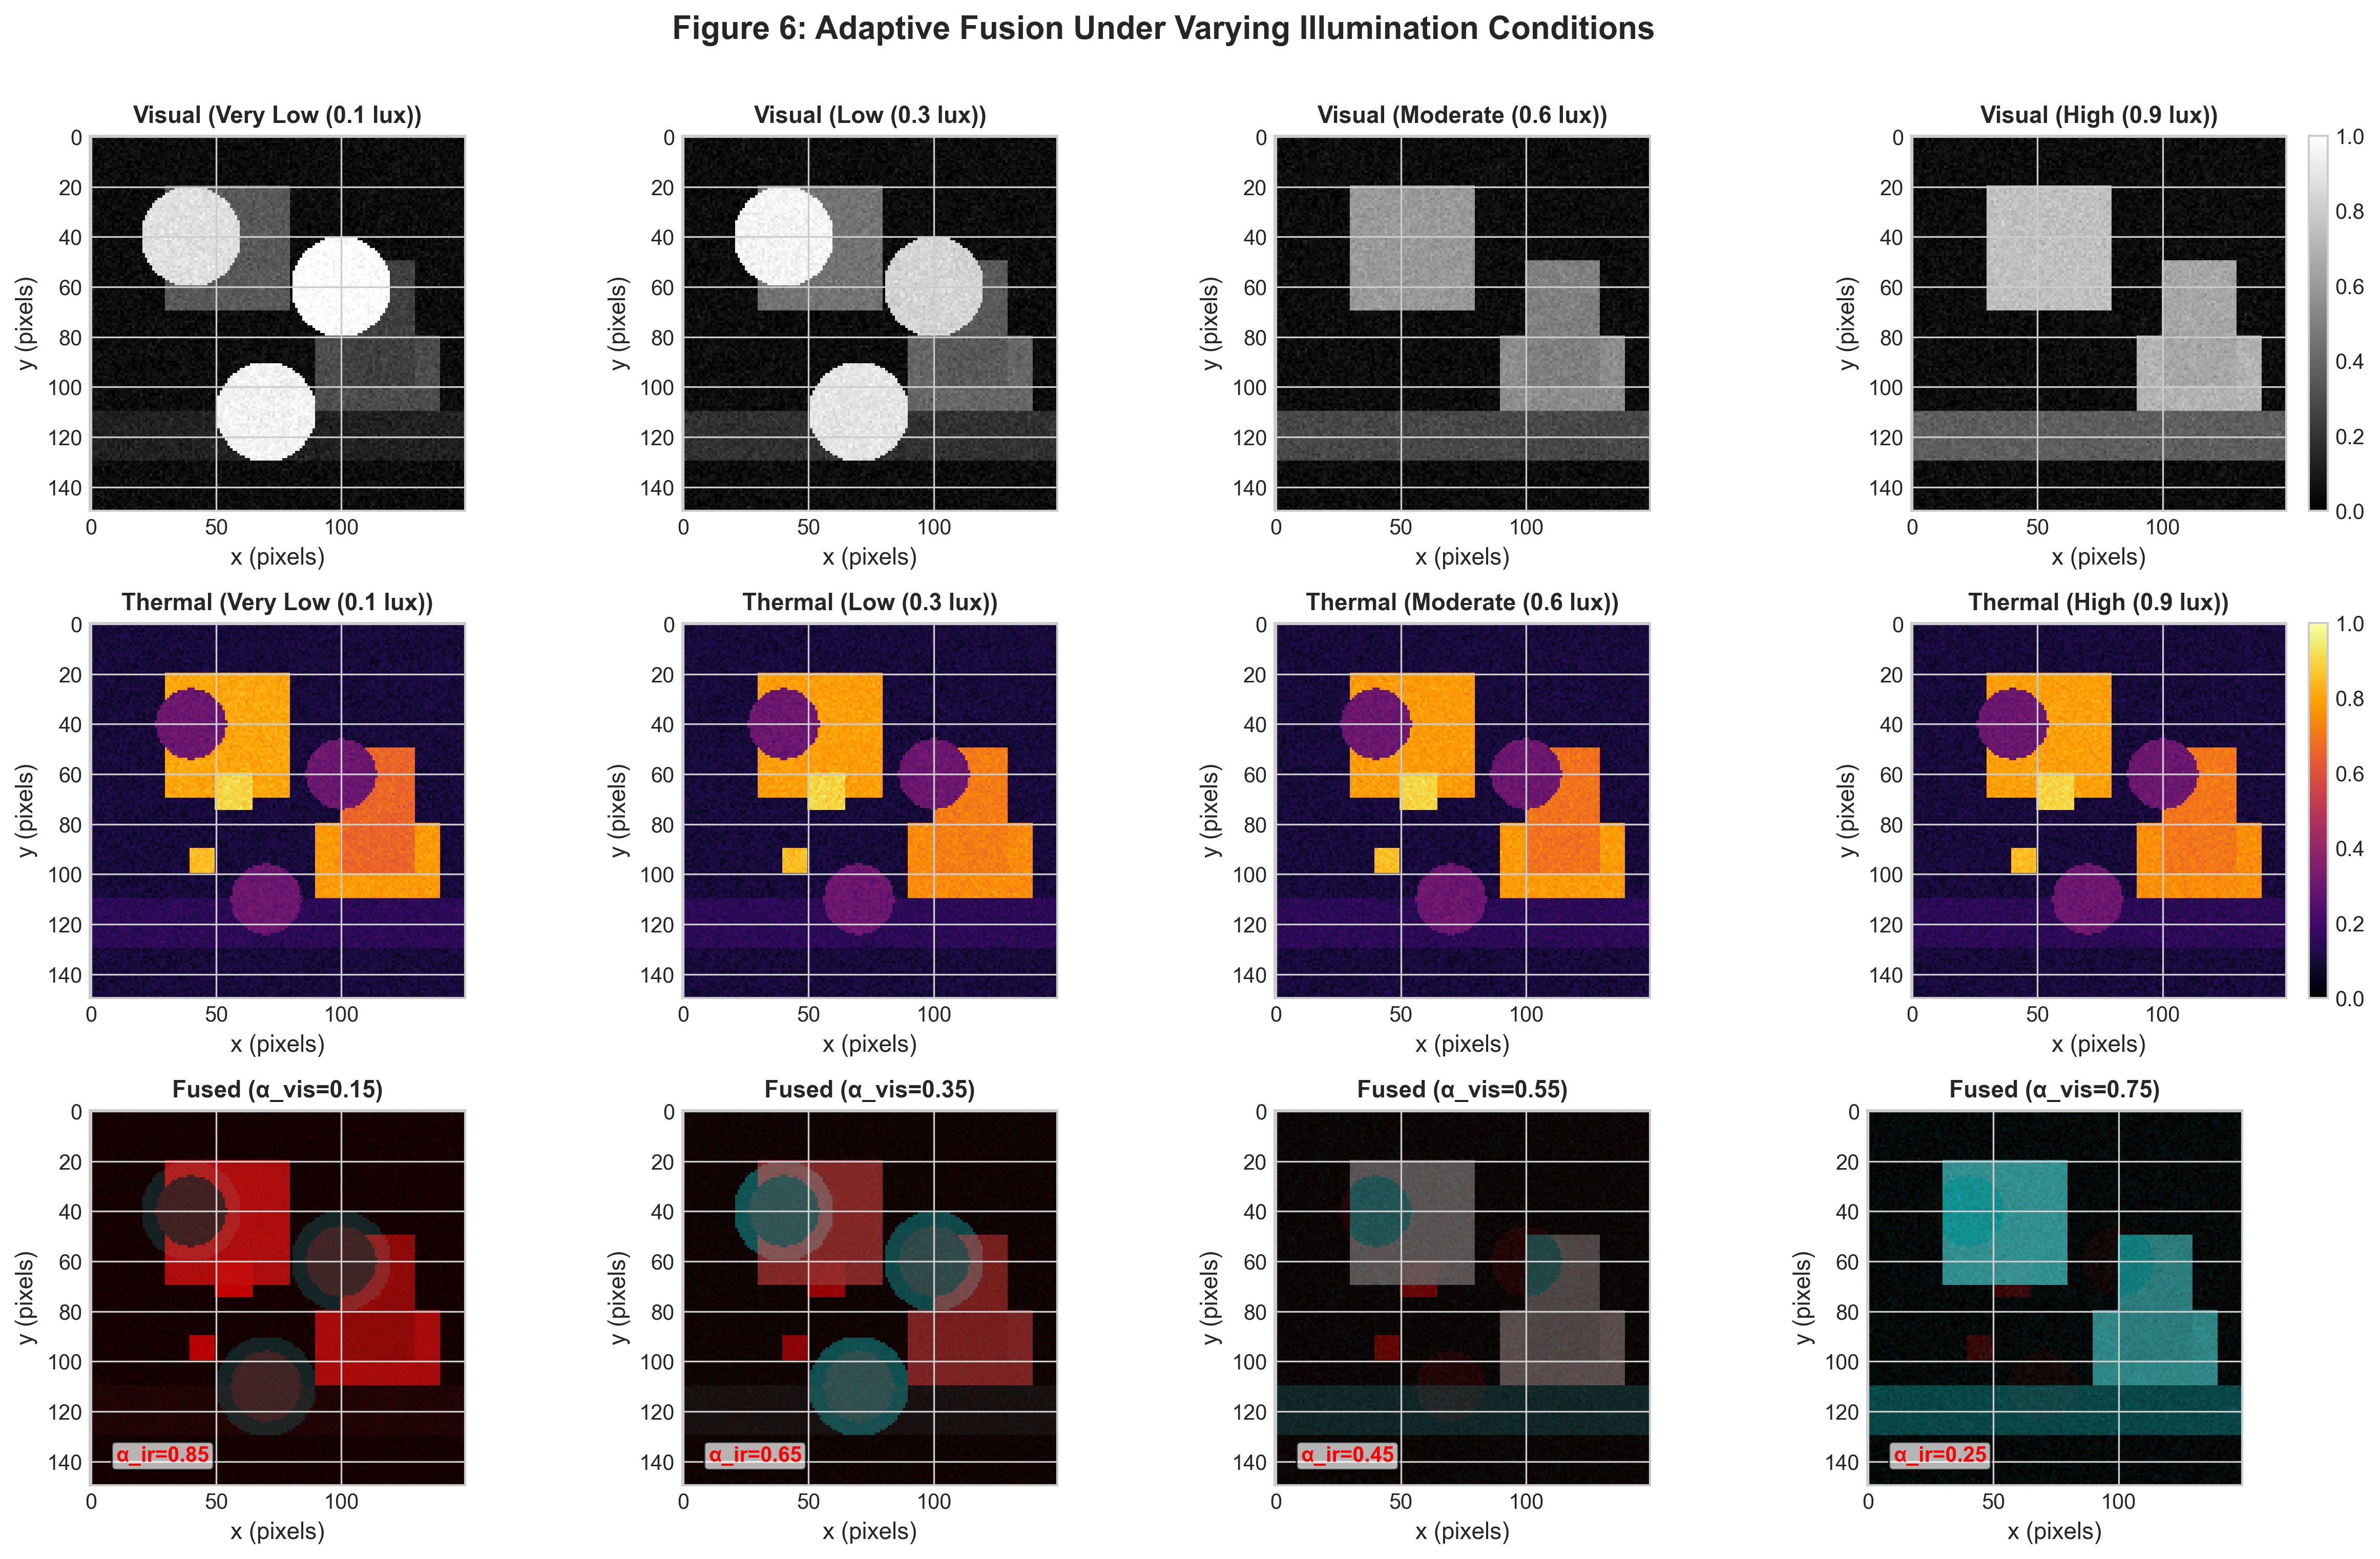
\includegraphics[width=0.98\columnwidth]{figures/fig_adaptive_fusion_example.png}
\caption{דוגמאות למיזוג אדפטיבי בארבע רמות תאורה שונות: 0.1, 0.5, 2, ו-50 לוקס. בכל שורה: תמונה חזותית (שמאל), תמונה תרמית (אמצע), ותמונה ממוזגת (ימין). (Adaptive fusion examples at four illumination levels: 0.1, 0.5, 2, and 50 lux. Each row: visual image (left), thermal image (center), and fused image (right).)}
\label{fig:ch05_adaptive_example}
\end{figure}

איור~\ref{fig:ch05_adaptive_example} מדגים את התנהגות מנגנון המיזוג האדפטיבי. בתאורה גבוהה (50 לוקס), התמונה הממוזגת דומה מאוד לתמונה החזותית, תוך שימור פרטים עדינים. בתאורה נמוכה (0.1 לוקס), התמונה הממוזגת שואבת בעיקר מהתמונה התרמית, תוך הוספת מידע מרקם מוגבל מהתמונה החזותית.

\subsection{סיכום}
\label{sec:ch05_summary}

בפרק זה הצגנו מסגרת מיזוג רב-שכבתית המשלבת מידע ממצלמה חזותית ומצלמה תרמית בשלוש רמות שונות. מנגנון הקשב הצולב מאפשר לרשת ללמוד קורלציות מודאליות-חוצות בקני מידה מרחביים שונים, ומנגנון המיזוג האדפטיבי מתאים את משקל התרומה של כל חיישן בהתאם לתנאי התאורה. התוצאות מראות שיפור משמעותי באיכות התמונה הממוזגת, עם SSIM של 0.87 לעומת 0.78 בשיטות קיימות.